\documentclass[main.tex]{subfiles}
\begin{document}
\author{Philipp Nickel}
\section{Der Datensatz CTU13}
\subsection{Herkunft}
Der CTU-13 ist ein Datensatz aus Botnet Traffic, welcher von der Czech Technical University in Prag, im Jahr 2011 aufgezeichnet wurde. 
\subsection{Struktur}
Das Ziel der Aufzeichnung war es einem großen Datensatz von realem Botnet Traffic vermischt mit normalem und background Traffic zu erstellen. Insgesamt besteht der Datensatz aus 13 Aufzeichnungen (Weiterführend als Szenarios bezeichnet). In jedem Szenario wurden spezifische Malware ausgeführt. Diese Malware nutzten unterschiedliche Protokolle und führten verschiedene Aktionen aus.  \\
In der Folgenden Tabelle ist genauer beschrieben, in welchen Szenarien IRC, P2P oder HTTP Protokolle benutzt wurden, sowie ob SPAM gesendet wurde, Click-Fraud oder DDos Angriffe betrieben wurden, Ports gescannt wurden oder Fast-Flux Techniken angewandt wurden oder custom compiliert wurde.\\
\begin{center}
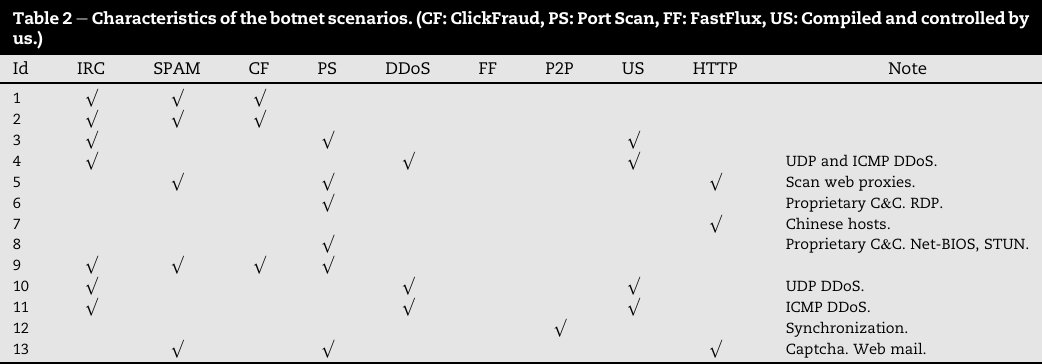
\includegraphics[scale=1]{images/CTU_Tabelle_1.jpg} 
\label{Tabelle: Charakteristika der Szenarien}
\end{center}
 % Quelle http://mcfp.weebly.com/the-ctu-13-dataset-a-labeled-dataset-with-botnet-normal-and-background-traffic.html
\\
In der folgenden Tabelle können Sie die Aufzeichnungsdauer der einzelnen Szenarien, die Anzahl der Packete, Anzahl an Netflows und die Größe der pcap Datei einsehen. Zusätzlich enthält die Tabelle die in den Szenarios benutzte Malware und die Anzahl an infizierten Rechnern.  
% Bild Tabelle einfügen
\begin{center}
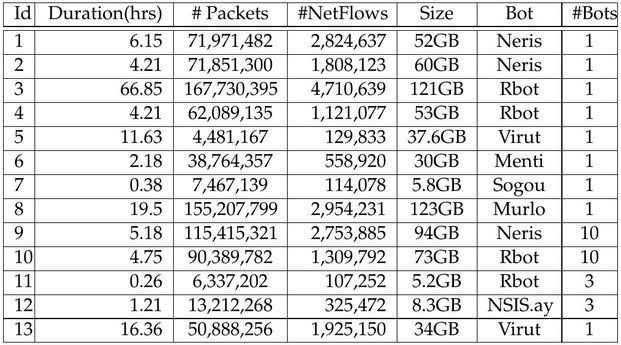
\includegraphics[scale=1]{images/CTU_Tabelle_2.jpg} 
\label{Tabelle: Größe der Daten für jedes Szenario}
% Quelle http://mcfp.weebly.com/the-ctu-13-dataset-a-labeled-dataset-with-botnet-normal-and-background-traffic.html
\end{center}
Die finale NetFlow Datei besteht aus folgenden Feldern:
\begin{center}
\begin{enumerate}
\item Start Time
\item End Time
\item Duration
\item Source IP address
\item Source Port
\item Direction
\item Destination IP address
\item Destination Port
\item State
\item SToS
\item Total Packets
\item Total Bytes
\end{enumerate}
\end{center}
Insgesamt umfasst der CTU-13 Datensatz bis zu 662.9 GB an pcap Dateien.  \\
\subsection{Besonderheiten}
Der CTU13-Datensatz enthält im Vergleich zu anderen Datensätzen einige Besonderheiten. Diese Besonerheiten werden im Verlauf dieses Kapitels genauer erläutert.
\subsubsection{Label}
% Besonderheit der Labels: Botnet, background, normal
Während der Erstellung des Datensatzes wurden 3 verschiedene Labels vergeben: Background, Botnet und Normal. Diese wurden nach folgender Priorität vergeben: 
\begin{center}
\begin{enumerate}
\item Dem gesamten Traffic das Background Label zuordnen
\item Das Normal Label Traffic zuordnen, welcher bestimmten Filtern entspricht
\item Jedem Traffic das Label Botnet zuordnen, welcher von oder zu einer bekannten infizierten IP Adresse kommt
\end{enumerate}
\end{center}
Die genutzten Filter wurden von bekannten und kontrollierten Computer im Netzwerk, wie Routern, Proxies, Switches und eigenen Laborrechnern erstellt.
\subsubsection{Bidirectional Netflow}
In dem im Projekt benutztem CTU-13 Datensatz enthält bidirectional NetFlows. Diese bidirectional NetFlows haben gegenüber directional NetFlows folgende Vorteile: 
\begin{center}
\begin{enumerate}
\item Das Problem der Differentierung zwischen Client und Server wird damit gelöst.
\item Sie enthalten mehr Informationen
\item Sie enthalten detailliertere Labels.
\end{enumerate}
\end{center}
\subsubsection{Manuell gelabelt}
Die Szenarios des CTU-13 Datensatzes wurden manuell analysiert und gelabelt. Der Prozess der Labelverteilung erfolgte innerhalb der NetFlow Dateien.
\subsubsection{NetFlow}
Zur weiteren Verwendung und Analyse des CTU-13 Datensatzes stehen die kompletten pcap Dateien aus Datenschutzgründen nicht zur Verfügung.
\subsection{Entscheidung}

\end{document}

%Woher kommt dieser Datensatz/ Wie ist er entstanden?
%Welche Struktur weist er auf?
%Welche Besonderheiten gibt es? (z.B. Backgroundtraffic)
%Warum haben wir gerade diesen Datensatz gewählt?

